\documentclass{beamer}
\usepackage[noindent]{ctex}
\usetheme{Madrid}
\title{一种改进的回答集逻辑程序分割方法 \\ 及程序化简研究}
\author{霍子伟}
\institute{中山大学软件学院}
\setbeamertemplate{navigation symbols}{}
\setbeamertemplate{frametitle}
{
    \begin{beamercolorbox}[sep=0.2cm,ht=1.8em,wd=\paperwidth]{frametitle}
        \insertframetitle
    \end{beamercolorbox}
}
\begin{document}

\titlepage


\begin{frame}[t]{主要内容}
	\begin{itemize}
		\item {研究背景}
		\item {改进的程序分割方法
%			\begin{itemize}
%				\item NLP的新程序分割方法
%				\item DLP的新程序分割方法
%				\item 强程序分割方法
%				\item 计算复杂性分析
%			\end{itemize}
			}
		\item {程序化简}
		\item {实验与分析
%			\begin{itemize}
%				\item 实验环境
%				\item 程序分割实验
%				\item 程序化简实验
%			\end{itemize}
			}
		\item {总结与展望
%			\begin{itemize}
%				\item 研究总结
%				\item 研究展望
%			\end{itemize}
			}
	\end{itemize}
\end{frame}


%%%%%%%%%%%%%%%%%  研究背景  %%%%%%%%%%%%%%%%%
\begin{frame}[t]{研究背景}
	\begin{enumerate}
		\item 什么是ASP逻辑程序
		\item 分割集和程序分割方法
%		\item 分割理论的应用
	\end{enumerate}
\end{frame}


\begin{frame}[t]{什么是ASP逻辑程序}
	% 根据发展历史来引出ASP
	ASP逻辑程序形成与发展历史:
	\begin{itemize}
		\item 70年代,Kowalski提出逻辑可以作为程序语言的基础的观点
		\item 1978年,Clark提出失败即否定和Clark完备
		\item 1979年,Colmerauer发明了第一种逻辑程序语言:PROLOG
		\item 1988年,Gelfond和Lifschitz提出稳定模型语义
		\item 90年代,回答集编程(ASP : Answer Set Program)形成
		\item 90年代至今,一系列ASP求解器诞生,ASP语义也在不断扩展
	\end{itemize}
\end{frame}


\begin{frame}[t]{什么是ASP逻辑程序}
	% 根据发展历史来引出ASP
	ASP逻辑程序形成与发展历史:
	\begin{itemize}
		\item 70年代,Kowalski提出逻辑可以作为程序语言的基础的观点
		\item 1978年,Clark提出失败即否定和Clark完备
		\item 1979年,Colmerauer发明了第一种逻辑程序语言:PROLOG
		\item 1988年,Gelfond和Lifschitz提出稳定模型语义
		\item 90年代,回答集编程(ASP : Answer Set Program)形成
		\item 90年代至今,一系列ASP求解器诞生,ASP语义也在不断扩展
	\end{itemize}
	

	\textbf{ASP中的一个研究热点是:ASP求解的提速。}
	% 而1994年,Lifschitz和Turner提出的分割理论就是给ASP求解提速的一个方法
	
\end{frame}


\begin{frame}[t]{分割集和程序分割方法}
	% Lifschitz和Turner分割集和程序分割方法
	\begin{itemize}
		\item \textbf{分割集(Splitting Set):}给定一个ASP逻辑成$P$,其分割集时一个原子集$U$,$U$满足:对于任意的规则$r \in P$有$head(r) \cap U \neq \emptyset$蕴涵$Atoms(r) \subseteq U$。
		\item {\textbf{底部和顶部(bottom \& top):}标记$P$关于$U$的底部为$b_U(P)$,顶部为$t_U(P)$,并定义为:
			\begin{itemize}
				\item $b_U(P) = \{ r \in P~|~head(r) \cap U \neq \emptyset \}$
				\item $t_U(P) = P~\backslash~b_U(P)$
			\end{itemize}
			}
		\item {\textbf{化简操作$e_U(P,X)$:}其中$X$为原子集,对$P$执行以下两个步骤:
			\begin{itemize}
				\item 删除符合以下条件的规则$r$:$head(r) \cap X \neq \emptyset$且$body^+(r) \cap U \nsubseteq X$,或者$(body^-(r) \cap U) \cap X \neq \emptyset$;
				\item 在剩下的规则的体部中把所有形如$a$或$not~a$的文字删掉,其中$a \in U$。
			\end{itemize}
			}
	\end{itemize}
	
\end{frame}


\begin{frame}[t]{分割集和程序分割方法}
	\begin{itemize}
		\item {\textbf{方案(Solution):} $P$关于$U$的一个方案是一组原子集$\langle X,Y \rangle$,具体地:
			\begin{itemize}
				\item $X$是$b_U(P)$的回答集;
				\item $Y$是$e_U(P \backslash b_U(P), X)$的回答集。
			\end{itemize}
			}
	\end{itemize}
	
	
	\begin{theorem}[分割集理论]
		已知ASP逻辑程序$P$和其分割集$U$,则一个原子集$S$是$P$的回答集,当且仅当$S = X \cup Y$,其中$\langle X,Y \rangle$是$P$关于$U$的一个方案。
	\end{theorem}
	
\end{frame}


\begin{frame}[t]{分割集和程序分割方法}
	\begin{itemize}
		\item {\textbf{方案(Solution):} $P$关于$U$的一个方案是一组原子集$\langle X,Y \rangle$,具体地:
			\begin{itemize}
				\item $X$是$b_U(P)$的回答集;
				\item $Y$是$e_U(P \backslash b_U(P), X)$的回答集。
			\end{itemize}
		}
	\end{itemize}
	
	
	\begin{theorem}[分割集理论]
		已知ASP逻辑程序$P$和其分割集$U$,则一个原子集$S$是$P$的回答集,当且仅当$S = X \cup Y$,其中$\langle X,Y \rangle$是$P$关于$U$的一个方案。
	\end{theorem}
	
	\vspace{0.5cm}
	
	\textbf{局限性}:
	\begin{itemize}
		\item 对于大部分程序,其分割集是:$\emptyset$或$Atoms(P)$
	\end{itemize}
	
\end{frame}


% 分割理论的应用
%\begin{frame}[t]{分割理论的应用}
%	分割理论的具体应用例子:
%	\begin{itemize}
%		\item 2008年,Gebser以分割集理论作为基础实现了增量式ASP求解器――iclingo;
%		\item 2008年,Oikarinen和Janhunen把分割集的思想拓展到了带嵌套表达式的逻辑程序中;
%		\item 2009年,Ferraris则在稳定模型语义下的任意一阶逻辑中引入了分割集的使用。
%	\end{itemize}
%\end{frame}


%%%%%%%%%%%%%%%%%%%%%%%%%%%%%%%%%%%%%%%%%%%%%

%%%%%%%%%%%%%%%% 改进的程序分割方法 %%%%%%%%%%%%%
\begin{frame}[t]{改进的程序分割方法}
	\begin{enumerate}
		\item NLP的新程序分割方法
		\item DLP的新程序分割方法
		\item 强程序分割方法
		\item 计算复杂性分析
	\end{enumerate}
\end{frame}


\begin{frame}[t]{NLP的新程序分割方法}
\end{frame}

%%%%%%%%%%%%%%%%%%%%%%%%%%%%%%%%%%%%%%%%%%%%%







\begin{frame}{数据类型}

\begin{figure}
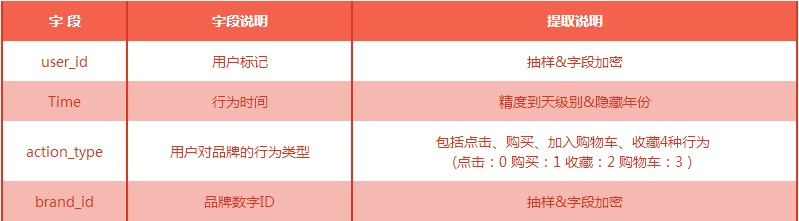
\includegraphics[width=\linewidth]{./data_info}
\end{figure}

\begin{itemize}
\item 用户对任意商品的行为都会映射为一行数据。
\item 其中所有商品ID都已汇总为商品对应的品牌ID
\item 用户和品牌都分别做了一定程度的数据抽样,且数字ID都做了加密
\item 所有行为的时间都精确到天级别(隐藏年份)
\end{itemize}

\end{frame}

\begin{frame}{数据类型}

\begin{figure}
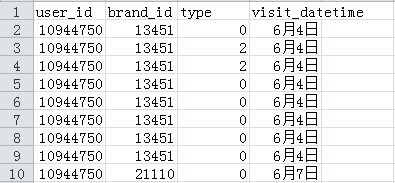
\includegraphics{./data_details}
\end{figure}

第一阶段的数据规模:
\begin{itemize}
\item 总条数:182880
\item 用户数:884
\item 品牌数:9531 
\end{itemize}

\end{frame}

\begin{frame}{评估指标:$F_1$-Score}

\begin{columns}[c]

\begin{column}{0.5\textwidth}
准确率:$precision = \frac{\sum_i^N hitBrands_i}{\sum_i^N pBrands_i}$

\vspace{1em}

注:
\begin{itemize}
\item $N$为参赛队预测的用户数
\item $pBrands_i$为用户$i$预测他(她)会购买的品牌列表个数 
\item $hitBrands_i$对用户$i$预测的品牌列表与用户$i$真实购买的品牌交集的个数
\end{itemize}
\end{column}

\begin{column}{0.5\textwidth}
召回率:$recall = \frac{\sum_i^M hitBrands_i}{\sum_i^M bBrands_i}$

\vspace{1em}

注:
\begin{itemize}
\item $M$为实际产生成交的用户数量
\item $bBrands_i$为用户$i$真实购买的品牌个数 
\item $hitBrands_i$预测的品牌列表与用户$i$真实购买的品牌交集的个数
\end{itemize}
\end{column}

\end{columns}

\vspace{1em}

\begin{center}
\zihao{4}
\colorbox{yellow}{$F_1$-Score: $F_1 = \frac{2 \times P \times R}{P + R}$}
\end{center}

\end{frame}

\begin{frame}{问题分析}

我们把该问题看作是一个\textcolor{red}{分类问题}——根据前4个月出现过的<user, brand>对的数据,来预测下一个月,该<user, brand>对是否发生购买

\vspace{1cm}

尝试过的做法:
\begin{itemize}
\item 基于矩阵分解的协同过滤(SVDFeature)
\item 基于规则的推荐
\item 多模型融合(规则、SVM\_Perf、 LR、 MLP、 SAE)
\end{itemize}

\end{frame}

\begin{frame}{方案1:SVDFeature}

SVDFeature是上海交大Apex实验室参加KDDCUP 2011期间开发的,可以完成feature-based matrix factorization。

\vspace{1em}

具体过程:
\begin{enumerate}
\item 将每个月的数据,构造成<user, brand>的矩阵(缺失的)$M_1, M_2, M_3, M_4$
\item 对每个月的矩阵使用SVDFeature进行矩阵补全,补全后的矩阵为$S_1, S_2, S_3, S_4$
\item 学习一个转移矩阵W($S_i$变换到$S_{i + 1}$)
\end{enumerate}

\end{frame}

\begin{frame}{方案1:SVDFeature}

\begin{figure}
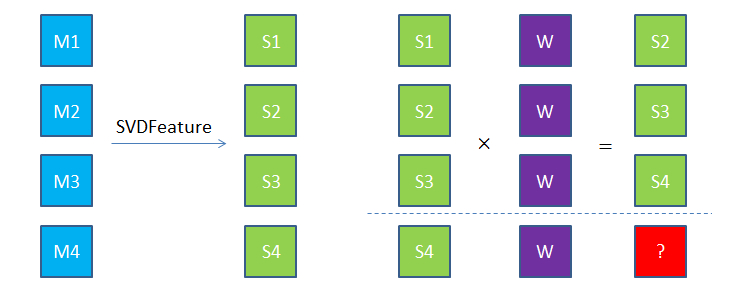
\includegraphics[width=0.8\linewidth]{./process}
\end{figure}

\vspace{-1em}

结果:效果不好,$F_1$-Score只有$0.09\%$

原因:
\begin{enumerate}
\item 数据规模小
\item 补全前的矩阵$M_1, M_2, M_3, M_4$过于稀疏
\item 无法处理“异常”的数据(如,购买/总操作数特别高的用户,只点击但是不购买的用户……)
\end{enumerate}

\end{frame}

\begin{frame}{方案2:基于规则的推荐}

我们设计了以下的规则:
\begin{enumerate}
\item 4个月所有的购买记录作为我们最后的预测($F_1\mbox{-Score}=5.41\%$)
\item 只出现在前2个半月购买,后面1个半月没有出现购买的<user, brand>对,我们把它\textcolor{red}{过滤}掉
\item 在最后的1个半月中,一个用户至少\textcolor{red}{\,\,\,5天点击}了该商品,并且他没有购买这个商品我们将该商品推荐给他
\item 在最后的1个半月中,一个用户\textcolor{red}{点击}某个商品\textcolor{red}{大于10次},并且他没有购买这个商品,我们将该商品推荐给他
\item 在最后的1个月中,一个用户在一天中\textcolor{red}{点击}某个商品\textcolor{red}{至少7次},并且\textcolor{red}{当天}他\textcolor{red}{没有购买}过别的商品,我们将该商品推荐给他
\end{enumerate}

\colorbox{yellow}{结果: $F_1$-Score $6.41\%$}

\end{frame}

\begin{frame}{方案3:多模型融合}

特征构造:
\begin{enumerate}
\item 对每个<user, brand>对按每一周分别统计点击、购买、收藏、加入购物车的总次数
\item 每个<user, brand>对的统计数据,按周依此排列成一行,每周有4个数据,分别对应点击总次数、购买总次数、收藏总次数、加入购物车总次数
\end{enumerate}

\vspace{1em}

例如:

用户$i$在第一周对品牌$j$一共点击了12次,购买了1次,在第二周对它点击了2次,收藏了3次,那么,
$<i, j>$对的前面8维分别是:

12 1 0 0 2 0 3 0

\end{frame}

\begin{frame}{方案3:多模型融合}

训练与预测的过程:
\begin{enumerate}
\item 训练集由2部分组成,第一部分是第1$\,\sim$12周的统计数据做为输入特征,第13$\,\sim$16周做为对应的Label;
第二部分是第3$\,\sim$14周的统计数据做为输入特征,第15$\,\sim$18周做为对应的Label
\item 对于前12周的一个<user, brand>对,如果在接下来的4周中出现购买记录,则对应的Label为1,反之对应的Label为0
\item 最后12周的统计数据做为预测用的输入特征,其输出的结果为我们最终的预测结果
\end{enumerate}

\end{frame}

\begin{frame}{方案3:多模型融合}

我们最终的模型是通过融合6个模型的结果得到的,其中包括:
\begin{itemize}
\item 两个MLP(多层感知机)
\item SAE(稀疏自编码网络)
\item LR(逻辑式回归)
\item svm\_perf
\item 基于规则的模型
\end{itemize}

\end{frame}

\begin{frame}{方案3:多模型融合}

\colorbox{yellow}{预处理:}由于正负样本不平衡,并且数据量少,因此需要复制正样本,使
得正负样本的数目大致平衡状态

\vspace{2em}

逻辑式回归:
\begin{itemize}
\item 结果:$precision = 6.49\%$
\end{itemize}

\vspace{1em}

svm\_perf:
\begin{itemize}
\item 该SVM算法有多种选项,可以让目标模型优化precision,或者优化$F_1$-Score
\item 估计结果:$precision = 7\%$
\end{itemize}

\end{frame}

\begin{frame}{方案3:多模型融合}

MLP(多层感知机)

\begin{columns}[c]

\begin{column}{0.5\linewidth}
\begin{figure}
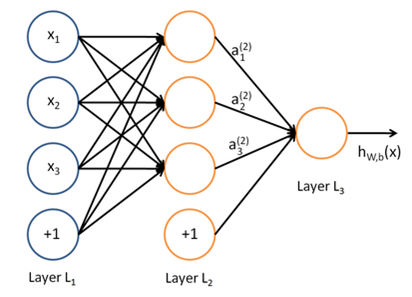
\includegraphics[width=\linewidth]{./MLP}
\end{figure}
\end{column}

\begin{column}{0.5\linewidth}
\begin{itemize}
\item 模型:三层网络结构,中间一层位隐含层(20个节点),输出层1个节点,采用交叉熵损失
\item 学习能力比LR强,可以学习到非线性的关系
\item {结果: \\$precision = 8\%$, $F_1\mbox{-Score} = 6.6\%$}
\end{itemize}
\end{column}

\end{columns}

\end{frame}

\begin{frame}{方案3:多模型融合}
SAE(自编码网络)

\begin{figure}
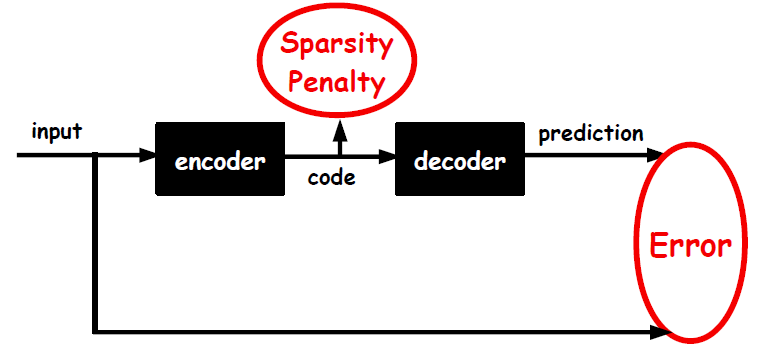
\includegraphics[width=0.5\linewidth]{./SAE}
\end{figure}

\begin{itemize}
\item 通过逐层学习自编码网络来初始化权重
\item 自编码是无监督的神经网络模型,通常加入稀疏性惩罚以学习到更有意义的特征
\item 模型:2层自编码编码层+1层sigmoid(softmax)输出层
\item 结果:$precision = 6.32\%$, $F_1\mbox{-Score} = 6.5\%$
\end{itemize}

\end{frame}

\begin{frame}{方案3:多模型融合}

融合的过程(\textcolor{red}{投票}):
\begin{enumerate}
\item 采用其中一个MLP模型(预测数目很少,但precision有$11.5\%$)作为基本的模型
\item 其他的5个模型,对其求差集
\item 对这5个差集中的<user, brand>对进行投票
\item 投票结果大于等于3的<user, brand>对合并上我们基本的模型就是我们最终所要预测的结果
\end{enumerate}

\colorbox{yellow}{结果:$F_1\mbox{-Score} = 6.74\%$}

\end{frame}

\begin{frame}{“天池”平台}

第二阶段的比赛规则是:参赛者须使用“天池”平台(阿里巴巴自主研发的分布式计算平台),访问海量的天猫数据,
并利用MapReduce、SQL及各种平台集成的机器学习算法包调试模型、提交结果。 

\vspace{1em}

举办方会提供一个虚拟机给参赛队伍,参赛队伍通过Windows的远程桌面连接便可登陆。

\end{frame}

\begin{frame}{“天池”平台}

ODPS(Open Data Processing Service)是阿里巴巴自主研发的海量数据离线数据处理平台。
主要服务于实时性要求相对不高的批量\textcolor{red}{结构化数据}的\textcolor{red}{储存}
和\textcolor{red}{计算},可以提供海量\textcolor{red}{数据仓库}的解决方案以及
针对大数据的\textcolor{red}{分析建模}服务。

\vspace{1em}

ODPS有许多的功能,我们这次比赛主要用到的是它所提供的\textcolor{red}{计算及分析任务}的功能:
\begin{itemize}
\item ODPS SQL
\item ODPS XLab/XLib
\item MapReduce
\end{itemize}

\end{frame}

\begin{frame}{ODPS SQL}

ODPS SQL采用的是类似于SQL的语法,可以看作是标准SQL的\textcolor{red}{子集},但\textcolor{red}{不能}因此
简单地把ODPS SQL\textcolor{red}{等价成}一个\textcolor{red}{数据库},它在很多方面并不具备数据库的特征,如
\textcolor{red}{事务}、\textcolor{red}{主键约束}等。

\vspace{1em}

从文档上也可以看出来,ODPS SQL的操作不支持单行的update和delete。(原因:实时性、吞吐量、容错……)

\vspace{1em}

\colorbox{yellow}{类似的开源软件:Hive}

\vspace{1em}

Hive是基于Hadoop的一个数据仓库工具,可以将结构化的数据文件映射为一张数据库表,并提供简单的SQL查询功能,
可以将SQL语句转换为MapReduce任务进行运行。

\end{frame}

\begin{frame}{ODPS SQL}

\begin{figure}
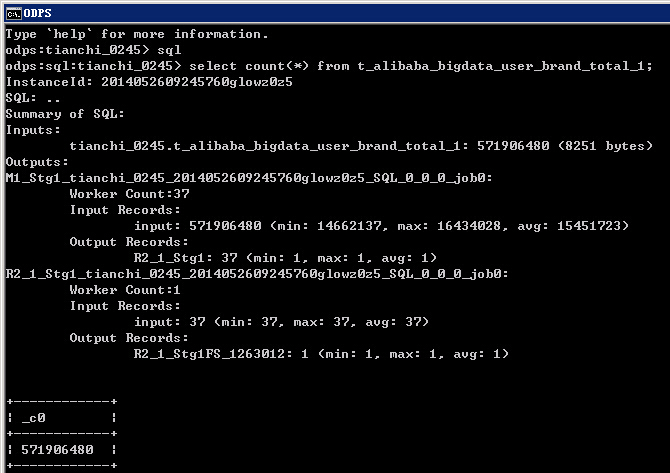
\includegraphics[width=0.9\linewidth]{./odps_query}
\end{figure}

\end{frame}

\begin{frame}{ODPS SQL}

通过ODPS SQL,我们可以知道第二阶段的数据规模为:

\begin{itemize}
\item 总条数:571906480
\item 用户数:12500984
\item 品牌数:29706 
\end{itemize}

\end{frame}

\begin{frame}{ODPS XLab/XLib}

XLab/XLib可以帮助用户轻松处理海量数据,包括了统计、机器学习、矩阵等常用计算功能。

\begin{itemize}
\item XLab是客户端。无论您是否有大数据分析的基础,都可以通过XLab\textcolor{red}{图形界面},轻松上手;
XLab还提供了\textcolor{red}{脚本编辑执行}功能,灵活方便、帮您成为大数据分析的高手。
\item XLib是XLab的后台\textcolor{red}{分布式算法库}。可以通过XLab或ODPS客户端调用;由于二者使用相同的
函数定义,XLab上的函数命令和脚本可以再ODPS客户端上执行执行。
\end{itemize}

\end{frame}

\begin{frame}{ODPS XLab/XLib}

\begin{figure}
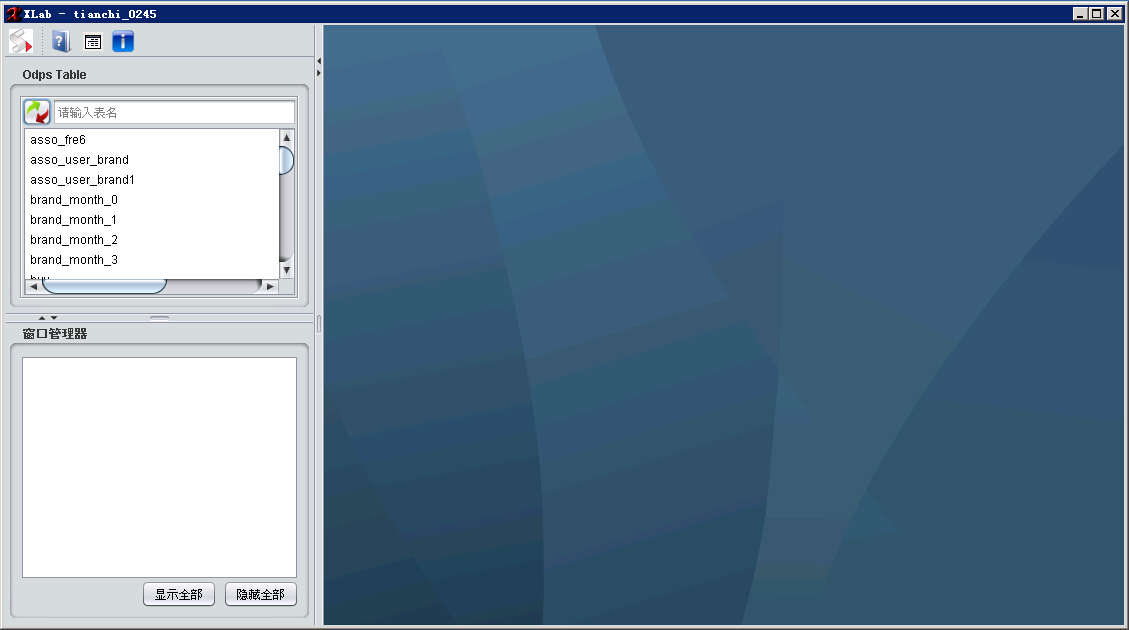
\includegraphics[width=\linewidth]{./XLab}
\end{figure}

\end{frame}

\begin{frame}{ODPS XLab/XLib}

\begin{figure}
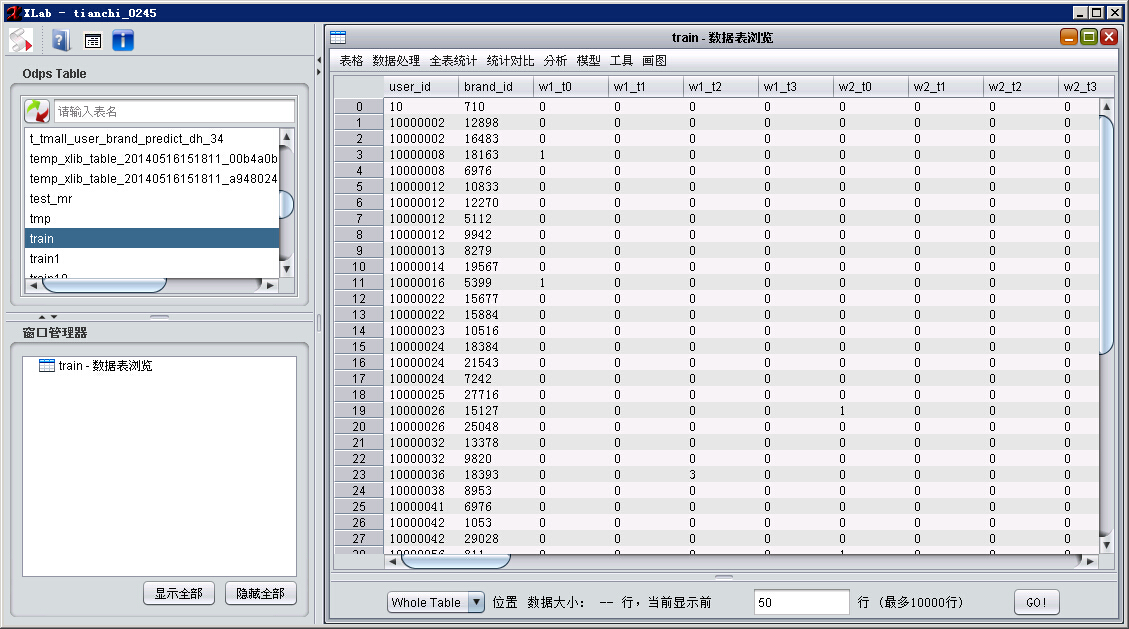
\includegraphics[width=\linewidth]{./XLab_table}
\end{figure}

\end{frame}

\begin{frame}{ODPS XLab/XLib}

\begin{figure}
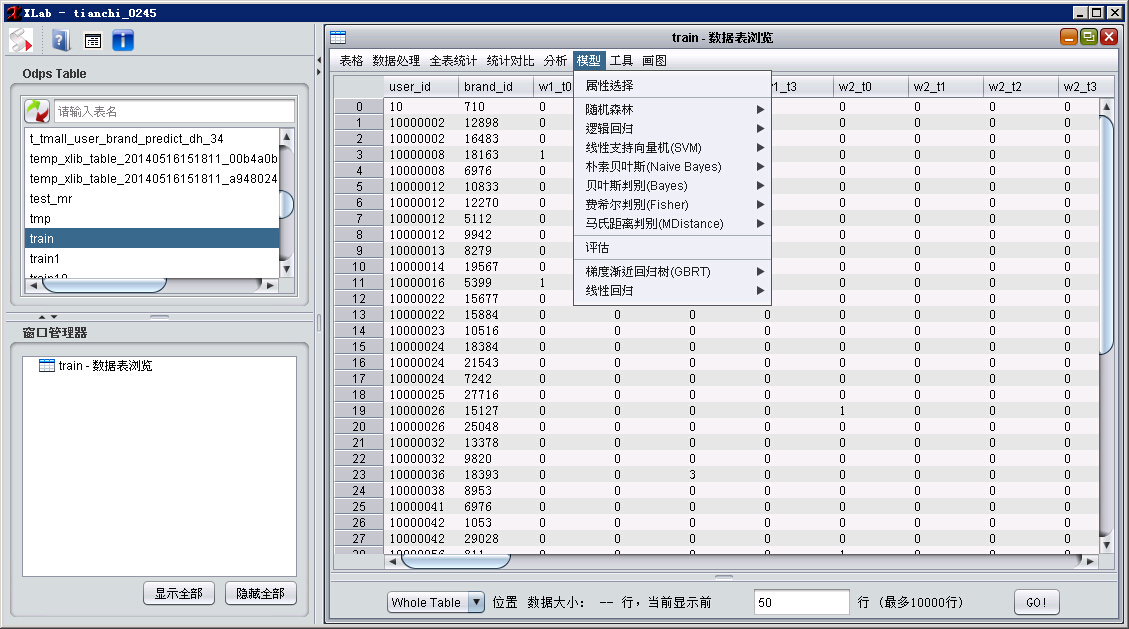
\includegraphics[width=\linewidth]{./XLab_models}
\end{figure}

\end{frame}

\begin{frame}{ODPS XLab/XLib}

\begin{figure}
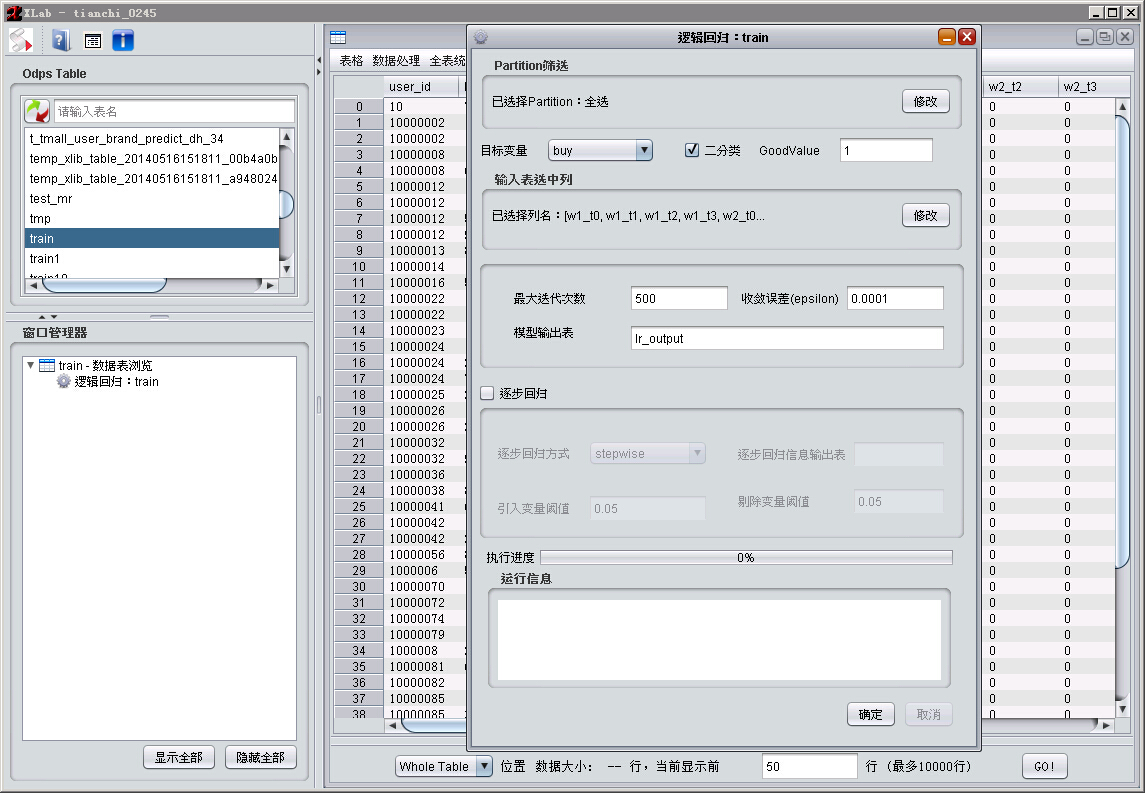
\includegraphics[width=0.9\linewidth]{./XLab_train}
\end{figure}

\end{frame}

\begin{frame}{ODPS XLab/XLib}

\begin{figure}
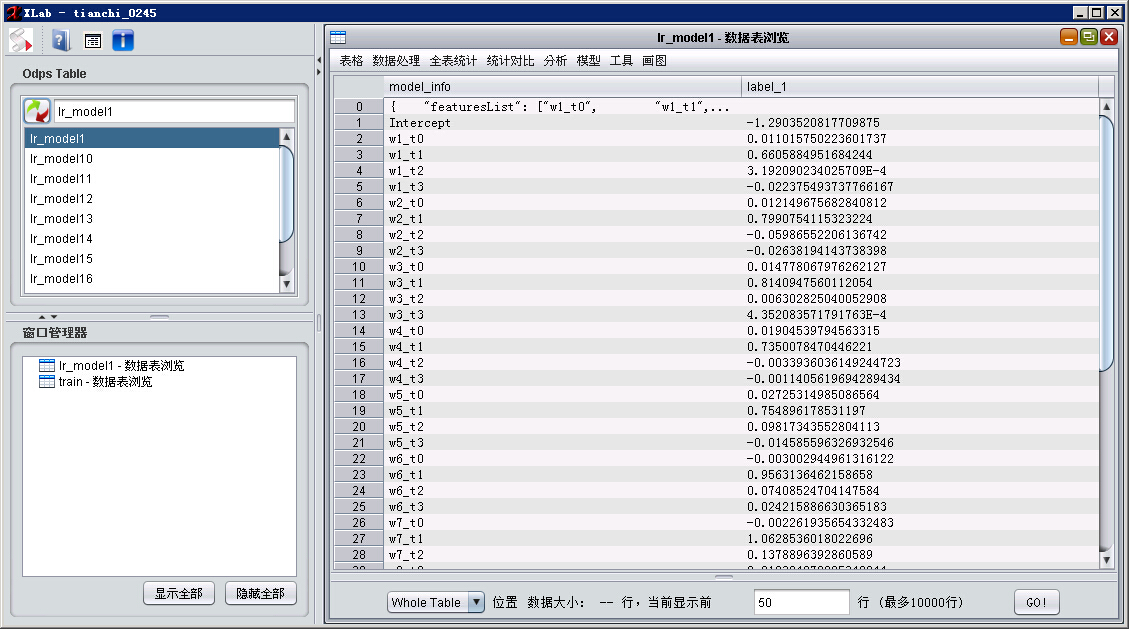
\includegraphics[width=\linewidth]{./XLab_result}
\end{figure}

\end{frame}

\begin{frame}{ODPS XLab/XLib}

\begin{figure}
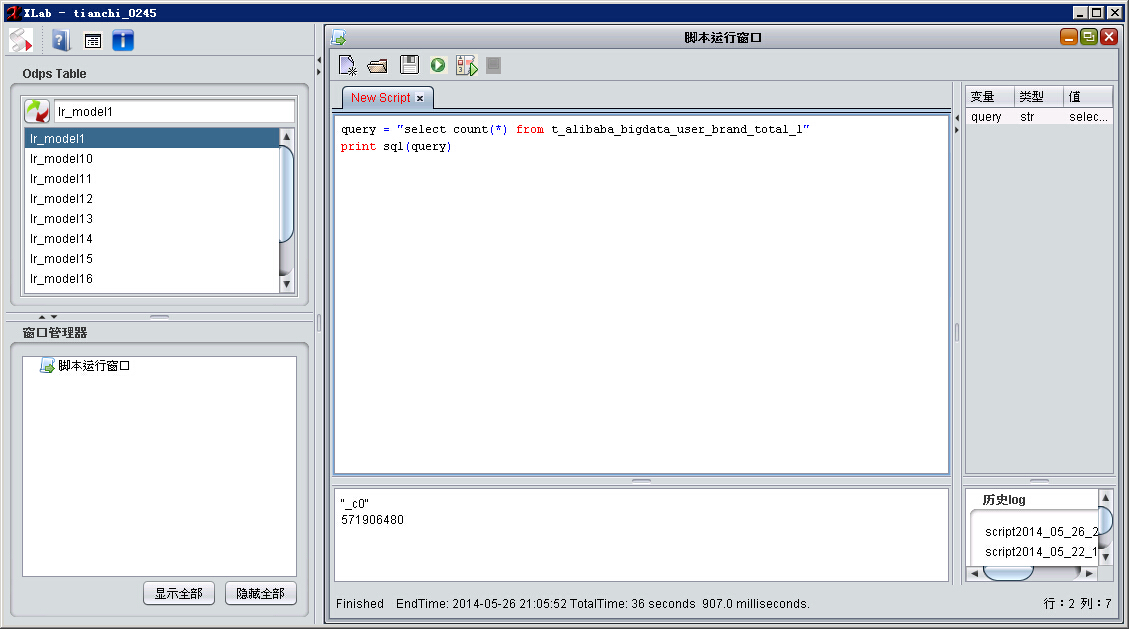
\includegraphics[width=\linewidth]{./XLab_script}
\end{figure}

\end{frame}

\begin{frame}{ODPS XLab/XLib}

\colorbox{yellow}{类似的开源软件:Mahout}

\vspace{1em}

Mahout 是 Apache Software Foundation(ASF) 旗下的一个开源项目,提供一些可扩展的机器学习领域经典算法的实现,
旨在帮助开发人员更加方便快捷地创建智能应用程序。

\vspace{1em}

Mahout包含许多实现,包括聚类、分类、推荐过滤、频繁子项挖掘。此外,通过使用 Apache Hadoop 库,Mahout 可以有效地扩展到云中。

\end{frame}

\begin{frame}{MapReduce}

\begin{figure}
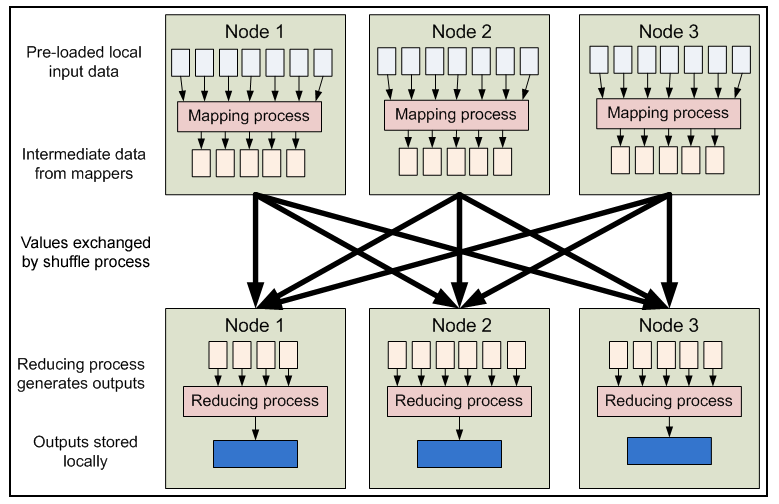
\includegraphics[width=0.75\linewidth]{./MapReduce_1}
\end{figure}

\vspace{-1em}

\begin{itemize}
\item 分布式并行计算框架,把大数据集分割成多个小数据集,分而治之,各个击破
\item 函数式编程范式,开发者需自定义map和reduce函数
\end{itemize}

\end{frame}

\begin{frame}{MapReduce}

\begin{figure}
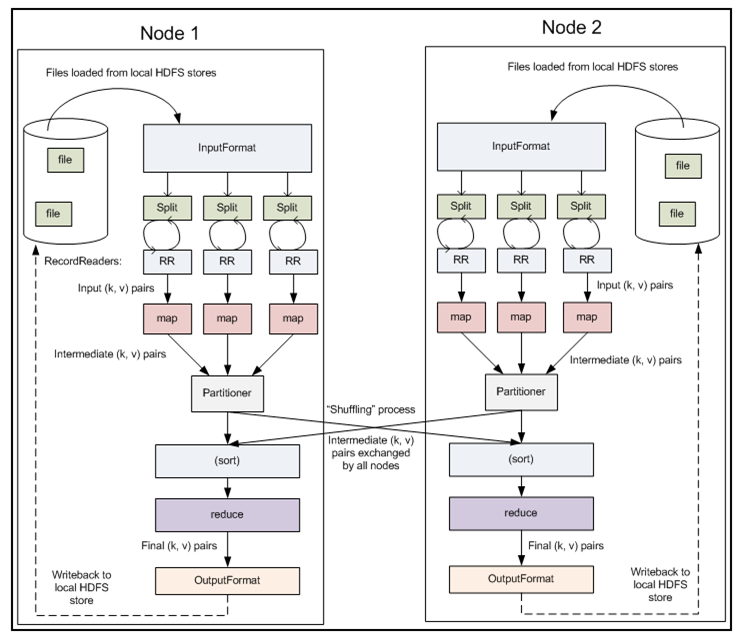
\includegraphics[width=0.95\linewidth]{./MapReduce_2}
\end{figure}

\end{frame}

\begin{frame}{MapReduce}

\begin{itemize}
\item 文件被划分为多个数据块存在HDFS文件系统中,每个Mapper取本地或靠近它的数据块进行map操作
\item MapReduce不支持修改数据
\item Mapper调用map处理文件的每一行数据,输入(k1, v1),输出(k2, v2)
\item Reducer调用reduce进行归约,输入(k, list of values)
\end{itemize}

\end{frame}

\begin{frame}{MapReduce Example: 统计词频}

\begin{figure}
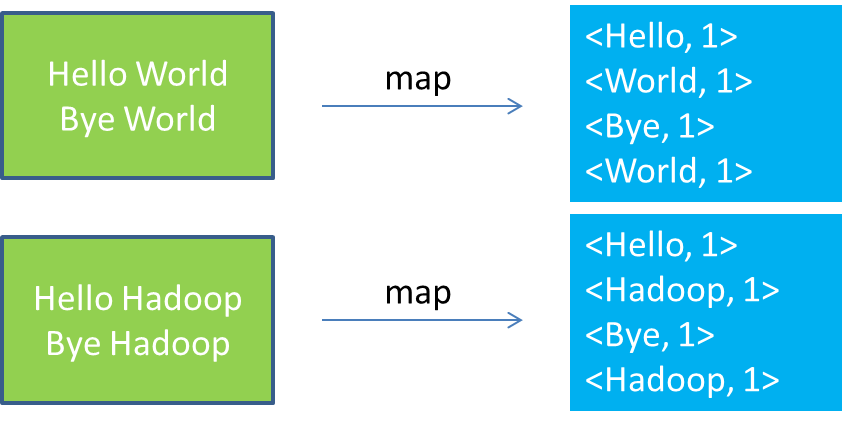
\includegraphics[width=\linewidth]{./WordCount_map}
\end{figure}

\end{frame}

\begin{frame}{MapReduce Example: 统计词频}

\begin{figure}
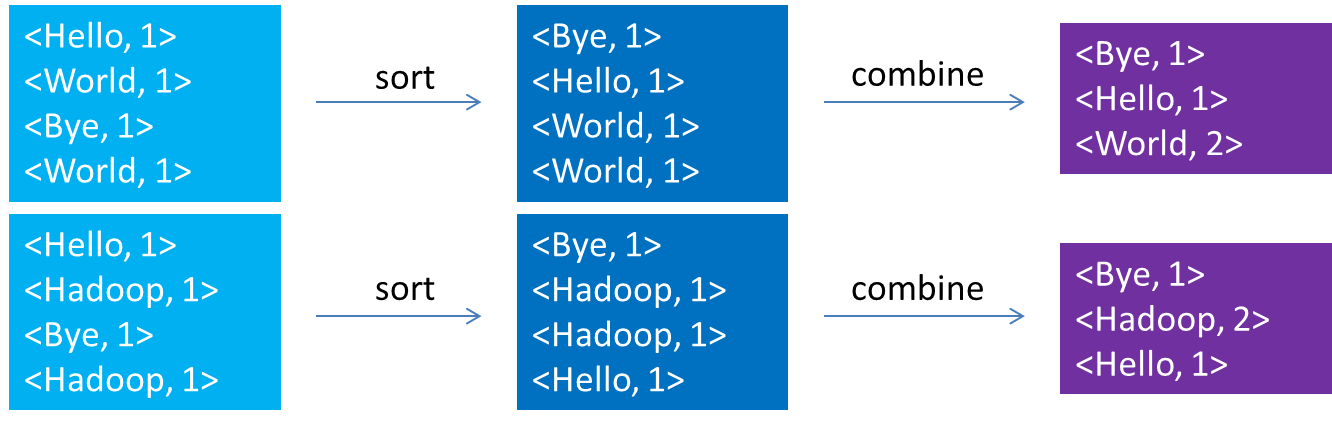
\includegraphics[width=\linewidth]{./WordCount_combine}
\end{figure}

\end{frame}

\begin{frame}{MapReduce Example: 统计词频}

\begin{figure}
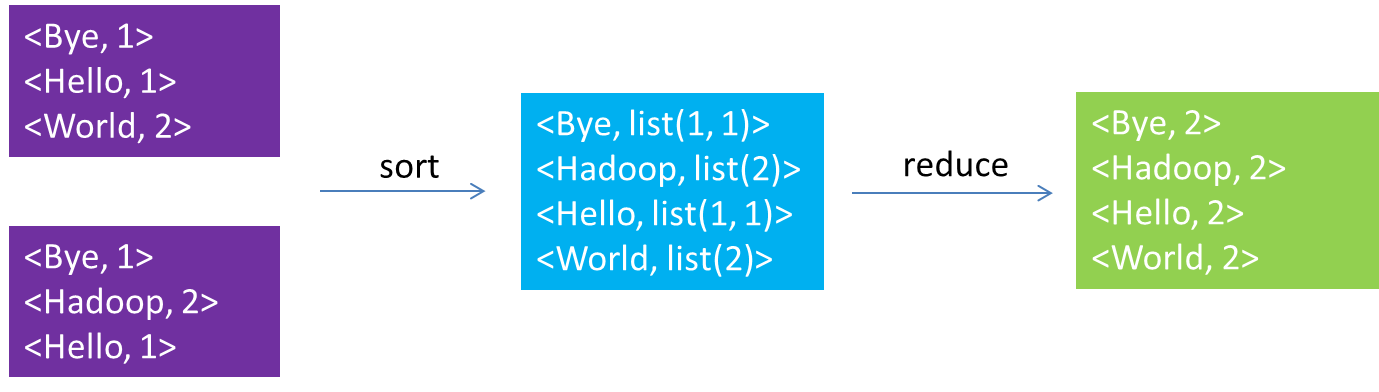
\includegraphics[width=\linewidth]{./WordCount_reduce}
\end{figure}

注:前面的sort-combine是在Mapper上做的,这里的sort-reduce是在Reducer上做的

\end{frame}

\begin{frame}{目前进展}

采取第$1 \sim 14$周的统计数据做为输入特征,第$15 \sim 18$周做为Label

\vspace{1em}

由于正负样本\textcolor{red}{极度不平衡},并且\textcolor{red}{数据量很大},
因此,我们对\textcolor{red}{负样本}进行\textcolor{red}{下采样},使得正负样本的数目
\textcolor{red}{大致平衡},以这样的方式训练50次,得到50个LR的模型,最后对这50个LR的模型求平均,得到我们最终的模型

\vspace{1em}

对预测结果抽取top 300万的数据做为我们最后的所提交的结果

\vspace{1em}

截止到今天的排名是156名。

\end{frame}

\begin{frame}{展望}

\begin{itemize}
\item 融入用户和商品特征,而不仅仅是行为序列特征
\item 尝试MLP、RF、GBDT等模型
\item 处理非平衡数据的另外方法:不抽样,带权重的损失函数
\item 推荐没有行为的商品:UserBased or ItemBased CF
\item 其他?
\end{itemize}

\end{frame}

\begin{frame}{感谢}

\zihao{-3}
感谢潘老师这2个多月来的指导,感谢刘冶师兄深夜帮忙跑模型,感谢在第一阶段的最后几天帮忙“扫雷”的同学!

\end{frame}

\end{document}